% !TeX program = xelatex
\documentclass[12pt,a4paper]{article}
\usepackage{fontspec}
\setmainfont{Times New Roman}[Path=C:/Windows/Fonts/,UprightFont=times.ttf,BoldFont=timesbd.ttf,ItalicFont=timesi.ttf,BoldItalicFont=timesbi.ttf]
\usepackage{amsmath,amssymb,amsfonts}
\usepackage[left=1.5cm,right=1.5cm,top=1.5cm,bottom=1.7cm,headheight=17pt]{geometry}
\usepackage{enumitem,array,graphicx,tikz,fancyhdr,needspace}
\usetikzlibrary{arrows.meta,calc,patterns}
% Sửa số đề và số trang đề thực tế sau khi biên dịch/tách PDF.
\newcommand{\soDe}{4}
\newcommand{\soTrangDe}{4}
\newcommand{\maDe}{\ifnum\soDe<1000 0\fi\ifnum\soDe<100 0\fi\ifnum\soDe<10 0\fi\soDe}
\pagestyle{fancy}
\fancyhf{}
\lhead{\small\textbf{ÔN TẬP GIỮA KÌ I}}
\rhead{\small\textit{Biên soạn: Dương Gia Bảo}}
\rfoot{\small Trang \thepage/\soTrangDe\ - Mã đề: \maDe}
\renewcommand{\headrulewidth}{0.4pt}
\fancypagestyle{answers}{\rfoot{\small Trang \thepage\ - Mã đề: \maDe}}
\fancypagestyle{firstpage}{\fancyhead{}\renewcommand{\headrulewidth}{0pt}}
\setlength{\parindent}{0pt}
\setlength{\parskip}{3pt}
\setlength{\emergencystretch}{1em}
\setlist[enumerate,1]{label=\textbf{Câu \arabic*:},leftmargin=*,itemsep=7pt,topsep=4pt}
\setlist[enumerate,2]{label=\alph*),leftmargin=*,itemsep=2.5pt,topsep=2.5pt}
\newcommand{\bonpa}[4]{\par\nobreak\smallskip\nobreak\noindent
\begin{tabular}{@{}p{0.47\linewidth}p{0.47\linewidth}@{}}
\textbf{A.} #1 & \textbf{B.} #2\\[8pt]
\textbf{C.} #3 & \textbf{D.} #4\end{tabular}}
\newcommand{\loigiai}[1]{\par\medskip\Needspace{4\baselineskip}\noindent\textbf{#1}\par\nobreak}
\newcommand{\otraloi}{\par\nobreak\smallskip\noindent\textit{Trả lời:}\quad\fbox{\rule{0pt}{11pt}\makebox[0.3cm]{}}\,\fbox{\rule{0pt}{11pt}\makebox[0.3cm]{}}\,\fbox{\rule{0pt}{11pt}\makebox[0.3cm]{}}\,\fbox{\rule{0pt}{11pt}\makebox[0.3cm]{}}}
\begin{document}
\thispagestyle{firstpage}
\noindent
\begin{minipage}[t]{0.35\textwidth}
    \centering
    {\fontsize{13}{15}\selectfont\textbf{ÔN TẬP GIỮA KÌ I}}\\[5pt]
    \textit{Biên soạn: Dương Gia Bảo}\\[6pt]
    \setlength{\fboxrule}{0.8pt}%
    \setlength{\fboxsep}{5pt}%
    \fbox{\begin{minipage}{0.83\linewidth}
        \centering
        {\fontsize{13}{15}\selectfont\textbf{ĐỀ ÔN TẬP}\\[2pt]\textbf{CHƯƠNG I VÀ II}}\\[5pt]
        \textit{(Đề thi gồm có \ifnum\soTrangDe<10 0\fi\soTrangDe\ trang)}
    \end{minipage}}
\end{minipage}\hfill
\begin{minipage}[t]{0.63\textwidth}
    \centering
    {\fontsize{13}{15}\selectfont\textbf{ÔN TẬP KIỂM TRA GIỮA KÌ I}\\[2pt]
    \textbf{NĂM HỌC 2026 - 2027}}\\[6pt]
    {\fontsize{14}{16}\selectfont\textbf{Môn: TOÁN - Lớp 12 (ĐỀ SỐ \soDe)}}\\[5pt]
    {\fontsize{11.5}{13}\selectfont\textit{Thời gian làm bài: 90 phút, không kể thời gian giao đề}}\\[6pt]
    \setlength{\fboxrule}{0.8pt}%
    \setlength{\fboxsep}{6pt}%
    \fbox{\makebox[3cm]{\fontsize{14}{16}\selectfont\textbf{Mã đề: \maDe}}}
\end{minipage}
\par\vspace{3pt}
\hrule height 0.6pt
\vspace{4pt}
\noindent\textit{Họ và tên học sinh:}\dotfill\hspace{1cm}\textit{Lớp:}\makebox[3.5cm]{\dotfill}
\par\vspace{3pt}
\hrule height 0.6pt
\vspace{4pt}

\vspace{2pt}
\section*{\large PHẦN I. Câu trắc nghiệm nhiều phương án lựa chọn}
\textit{Thí sinh trả lời từ câu 1 đến câu 12. Mỗi câu chỉ chọn một phương án.}
\begin{enumerate}
\item Cho hàm số $y=-x^3+3x^2+9x-2$. Hàm số đồng biến trên khoảng nào sau đây?
\bonpa{$(-1;3)$.}{$(-\infty;-1)$.}{$(3;+\infty)$.}{$(0;4)$.}

\item Cho hàm số $y=x^4-4x^2+3$. Số điểm cực trị của hàm số đã cho là
\bonpa{$1$.}{$2$.}{$3$.}{$0$.}

\item Giá trị nhỏ nhất của hàm số $f(x)=x^3-12x+1$ trên đoạn $[0;3]$ bằng
\bonpa{$1$.}{$-8$.}{$0$.}{$-15$.}

\item Tọa độ giao điểm $I$ của hai đường tiệm cận của đồ thị hàm số $y=\dfrac{3x+2}{x-2}$ là
\bonpa{$I(-2;3)$.}{$I(2;3)$.}{$I(3;2)$.}{$I(2;-2)$.}

\item Phương trình đường tiệm cận xiên của đồ thị hàm số $y=\dfrac{x^2-3x+5}{x-1}$ là
\bonpa{$y=x+2$.}{$y=x-2$.}{$y=2x-1$.}{$y=-x+2$.}

\Needspace{6\baselineskip}
\item Đường cong trong hình bên là đồ thị của hàm số nào dưới đây?
\par\nobreak\smallskip
\begin{minipage}[c]{0.60\linewidth}
\bonpa{$y=x^3-3x^2-1$.}{$y=-x^3+3x-1$.}{$y=x^3-3x+1$.}{$y=-x^3+3x^2-1$.}
\end{minipage}\hfill
\begin{minipage}[c]{0.36\linewidth}\centering
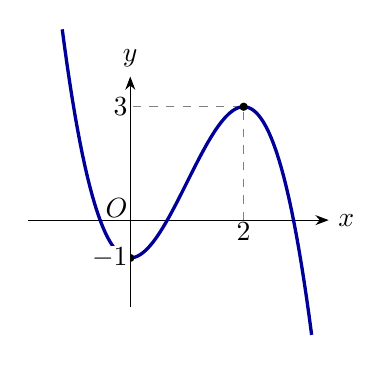
\begin{tikzpicture}[x=0.72cm,y=0.48cm,>=Stealth]
\draw[->] (-1.8,0)--(3.5,0) node[right] {$x$};
\draw[->] (0,-2.3)--(0,3.8) node[above] {$y$};
\draw[dashed,gray] (2,0)--(2,3)--(0,3);
\draw[very thick,blue!60!black,domain=-1.2:3.2,samples=100] plot (\x,{-\x*\x*\x + 3*\x*\x - 1});
\fill (0,-1) circle (1.5pt);\fill (2,3) circle (1.5pt);
\node[above left,fill=white,inner sep=0.8pt] at (0,0) {$O$};
\node[below,fill=white,inner sep=0.8pt] at (2,0) {$2$};
\node[left,fill=white,inner sep=0.8pt] at (0,3) {$3$};
\node[left,fill=white,inner sep=0.8pt] at (0,-1) {$-1$};
\end{tikzpicture}
\end{minipage}

\item Một chất điểm chuyển động theo phương trình $s(t)=-t^3+9t^2+t$, với $t$ tính bằng giây ($0\le t\le6$) và $s$ tính bằng mét. Vận tốc tức thời của chất điểm đạt giá trị lớn nhất tại thời điểm nào?
\bonpa{$t=2\text{ s}$.}{$t=4\text{ s}$.}{$t=3\text{ s}$.}{$t=5\text{ s}$.}
\end{enumerate}

\begin{enumerate}[start=8]
\item Cho hình hộp chữ nhật $ABCD.A'B'C'D'$. Đẳng thức vectơ nào sau đây đúng?
\bonpa{$\overrightarrow{AC'}=\overrightarrow{AB}+\overrightarrow{AD}+\overrightarrow{AA'}$.}{$\overrightarrow{AC'}=\overrightarrow{AB}+\overrightarrow{AC}+\overrightarrow{AA'}$.}{$\overrightarrow{AC'}=\overrightarrow{AB}+\overrightarrow{BC}+\overrightarrow{CD}$.}{$\overrightarrow{AC'}=\overrightarrow{A'B'}+\overrightarrow{A'D'}+\overrightarrow{AA'}$.}

\item Trong không gian $Oxyz$, cho hai điểm $M(2;-1;3)$ và $N(1;3;-2)$. Tọa độ của vectơ $\overrightarrow{MN}$ là
\bonpa{$(1;-4;5)$.}{$(3;2;1)$.}{$(-1;4;-5)$.}{$(-1;2;-5)$.}

\item Trong không gian $Oxyz$, cho hai vectơ $\vec u=(1;-2;3)$ và $\vec v=(3;1;-2)$. Tích vô hướng $\vec u\cdot\vec v$ bằng
\bonpa{$5$.}{$-1$.}{$1$.}{$-5$.}

\item Trong không gian $Oxyz$, cho hai điểm $A(1;2;-1)$ và $B(3;0;0)$. Khoảng cách giữa hai điểm $A$ và $B$ bằng
\bonpa{$3$.}{$\sqrt5$.}{$\sqrt3$.}{$9$.}

\item Trong không gian $Oxyz$, cho tam giác $ABC$ với $A(2;1;-3)$, $B(0;-2;5)$ và $C(4;4;1)$. Tọa độ trọng tâm $G$ của tam giác $ABC$ là
\bonpa{$(6;3;3)$.}{$(2;1;1)$.}{$(3;1;1)$.}{$(2;-1;1)$.}
\end{enumerate}

\section*{\large PHẦN II. Câu trắc nghiệm đúng hoặc sai}
\textit{Thí sinh trả lời từ câu 1 đến câu 4. Trong mỗi ý a), b), c), d), chọn đúng hoặc sai.}
\begin{enumerate}
\Needspace{8\baselineskip}
\item Cho hàm số $f(x)=\dfrac{x^2+3x+3}{x+2}$, xác định trên $\mathbb R\setminus\{-2\}$.
\begin{enumerate}
\item $f'(x)=\dfrac{x^2+4x+3}{(x+2)^2}$.
\item Hàm số nghịch biến trên khoảng $(-3;-1)$.
\item Đồ thị hàm số có đường tiệm cận xiên là $y=x+1$.
\item Đường thẳng đi qua hai điểm cực trị của đồ thị hàm số có phương trình là $y=2x+1$.
\end{enumerate}

\Needspace{8\baselineskip}
\item Một xưởng cơ khí sản xuất và bán hết $x$ sản phẩm mỗi tuần, với $x$ là số nguyên thỏa mãn $0\le x\le120$. Giá bán mỗi sản phẩm phụ thuộc vào số lượng sản xuất theo công thức $p(x)=600-3x$ (nghìn đồng). Tổng chi phí sản xuất trong tuần là $C(x)=x^2+80x+6000$ (nghìn đồng).
\begin{enumerate}
\item Doanh thu khi bán $x$ sản phẩm là $R(x)=-3x^2+600x$ (nghìn đồng).
\item Hàm lợi nhuận hàng tuần của xưởng là $P(x)=-4x^2+520x-6000$ (nghìn đồng).
\item Để thu được lợi nhuận lớn nhất, xưởng cần sản xuất và bán $70$ sản phẩm mỗi tuần.
\item Mức lợi nhuận lớn nhất mà xưởng có thể đạt được trong một tuần là $10{,}9$ triệu đồng.
\end{enumerate}
\end{enumerate}

\begin{enumerate}[start=3]
\item Trong không gian $Oxyz$, cho ba điểm $A(1;2;-1)$, $B(2;4;1)$ và $C(-1;3;2)$.
\begin{enumerate}
\item Tọa độ của vectơ $\overrightarrow{AB}$ là $(1;2;2)$ và có độ dài bằng $3$.
\item Tích vô hướng $\overrightarrow{AB}\cdot\overrightarrow{AC}=0$, tức tam giác $ABC$ vuông tại $A$.
\item Trọng tâm của tam giác $ABC$ là điểm $G\left(\dfrac23;3;\dfrac23\right)$.
\item Tọa độ đỉnh $D$ để tứ giác $ABCD$ là hình bình hành là $D(-2;1;0)$.
\end{enumerate}

\item Trong không gian $Oxyz$ (đơn vị trên các trục là mét), một chiếc đèn chùm có trọng lượng $P=60$ N được treo cân bằng bởi ba sợi dây cáp không giãn gắn vào trần nhà tại các điểm $A(-1;-\sqrt3;2)$, $B(-1;\sqrt3;2)$, $C(2;0;2)$ và cùng buộc vào đèn tại điểm $D(0;0;0)$. Đèn cân bằng khi tổng các vectơ lực tác dụng lên nó bằng $\vec0$. Trọng lực tác dụng lên đèn là $\vec P=(0;0;-60)$ N.
\begin{enumerate}
\item Độ dài của các đoạn dây $DA,DB,DC$ bằng nhau và bằng $2\sqrt2$ m.
\item Vectơ tổng $\overrightarrow{DA}+\overrightarrow{DB}+\overrightarrow{DC}=(0;0;6)$.
\item Lực căng tác dụng lên mỗi sợi dây có độ lớn bằng $20$ N.
\item Lực căng của sợi dây thứ ba biểu diễn dưới dạng tọa độ là $\vec T_3=(20;0;20)$ (đơn vị N).
\end{enumerate}
\end{enumerate}

\section*{\large PHẦN III. Câu trắc nghiệm trả lời ngắn}
\textit{Thí sinh trả lời từ câu 1 đến câu 6. Ghi kết quả vào các ô trả lời; dùng dấu phẩy cho phần thập phân.}
\begin{enumerate}
\item Có bao nhiêu giá trị nguyên của tham số $m$ thuộc đoạn $[-10;10]$ để hàm số $y=\dfrac{x-m}{x+3}$ đồng biến trên từng khoảng xác định của nó?
\otraloi

\item Trong không gian $Oxyz$, cho hình hộp $ABCD.A'B'C'D'$ có $A(2;1;-1)$, $B(4;2;0)$, $D(1;3;1)$ và $A'(3;-1;2)$. Biết tọa độ đỉnh $C'$ là $(a;b;c)$. Tính giá trị của biểu thức $S=a+b+c$.
\otraloi
\end{enumerate}

\newpage
\begin{enumerate}[start=3]
\item Từ một tấm tôn hình vuông cạnh $6$ dm, người ta cắt bỏ bốn hình vuông bằng nhau ở bốn góc có cạnh là $x$ dm rồi gấp phần còn lại thành một chiếc hộp không nắp. Bỏ qua độ dày tấm tôn. Thể tích lớn nhất của chiếc hộp bằng bao nhiêu dm$^3$?
\begin{center}
\begin{tikzpicture}[x=0.36cm,y=0.36cm,>=Stealth]
\fill[pattern=north east lines,pattern color=gray] (0,0) rectangle (1.2,1.2);
\fill[pattern=north east lines,pattern color=gray] (4.8,0) rectangle (6,1.2);
\fill[pattern=north east lines,pattern color=gray] (0,4.8) rectangle (1.2,6);
\fill[pattern=north east lines,pattern color=gray] (4.8,4.8) rectangle (6,6);
\draw[thick] (0,0) rectangle (6,6);
\draw[dashed] (1.2,0)--(1.2,6) (4.8,0)--(4.8,6) (0,1.2)--(6,1.2) (0,4.8)--(6,4.8);
\draw[<->] (0,-0.5)--(6,-0.5) node[midway,fill=white,inner sep=1pt] {$6\text{ dm}$};
\draw[<->] (6.5,0)--(6.5,6) node[midway,right] {$6\text{ dm}$};
\draw[<->] (0,6.5)--(1.2,6.5) node[midway,above] {$x$};
\node[font=\small] at (3,3) {Phần tôn giữ lại};
\end{tikzpicture}
\par\vspace{1pt}{\small\textit{Hình minh họa, không theo tỉ lệ.}}
\end{center}
\otraloi

\item Trong không gian $Oxyz$ (đơn vị trên các trục là kilômét), hai máy bay trực thăng xuất phát cùng lúc tại thời điểm $t=0$ (giờ). Vị trí của trực thăng thứ nhất tại thời điểm $t$ ($0\le t\le3$) là $A(2-t;1+t;3-t)$, vị trí của trực thăng thứ hai là $B(2+t;-2+3t;0)$. Khoảng cách nhỏ nhất giữa hai trực thăng trong khoảng thời gian này bằng bao nhiêu kilômét?
\otraloi

\item Một nhà máy sản xuất một loại hóa chất. Khi sản xuất $x$ tấn hóa chất trong một tháng ($5\le x\le50$), tổng chi phí sản xuất được mô hình hóa bởi $C(x)=x^3-12x^2+150x+800$ (triệu đồng). Chi phí trung bình trên mỗi tấn sản phẩm được xác định bởi $\overline{C}(x)=\dfrac{C(x)}{x}$ (triệu đồng/tấn). Hỏi nhà máy cần sản xuất bao nhiêu tấn hóa chất trong một tháng để chi phí trung bình trên mỗi tấn sản phẩm là nhỏ nhất?
\otraloi

\item Một người đang ở vị trí $A$ trên thuyền cách bờ biển thẳng một khoảng $AH=3$ km. Người đó muốn đến vị trí $B$ trên bờ biển cách $H$ một khoảng $HB=8$ km. Người đó chèo thuyền vào một điểm $M$ trên bờ biển ($M$ nằm giữa $H$ và $B$) với vận tốc $6$ km/h, sau đó chạy bộ từ $M$ đến $B$ với vận tốc $10$ km/h. Thời gian ngắn nhất để người đó đi từ $A$ đến $B$ bằng bao nhiêu giờ?
\par\nobreak\smallskip
\begin{minipage}[c]{0.35\linewidth}
\otraloi
\end{minipage}\hfill
\begin{minipage}[c]{0.62\linewidth}\centering
\begin{tikzpicture}[x=0.62cm,y=0.48cm,>=Stealth]
\draw[thick] (-0.3,0)--(8.5,0) node[right] {\footnotesize Bờ biển};
\fill[blue!10,opacity=0.6] (-0.3,-3.1) rectangle (8.5,0);
\node[blue!70!black,font=\footnotesize] at (1.2,-1.6) {\textit{Biển}};
\coordinate (A) at (0,-2.8);
\coordinate (H) at (0,0);
\coordinate (M) at (2.25,0);
\coordinate (B) at (8,0);
\draw[dashed] (A)--(H);
\draw[thick,red!80!black,->] (A)--(M) node[midway,below right,font=\footnotesize] {Chèo};
\draw[thick,teal!80!black,->] (M)--(B) node[midway,above,font=\footnotesize] {Chạy bộ};
\fill (A) circle (1.5pt) node[below] {\footnotesize $A$};
\fill (H) circle (1.5pt) node[above left] {\footnotesize $H$};
\fill (M) circle (1.5pt) node[above] {\footnotesize $M$};
\fill (B) circle (1.5pt) node[above] {\footnotesize $B$};
\draw (0.25,0)|-(0,0.25);
\draw[<->] (-0.4,-2.8)--(-0.4,0) node[midway,left,font=\footnotesize] {$3$};
\draw[<->] (0,-0.45)--(8,-0.45) node[midway,fill=white,inner sep=0.5pt,font=\footnotesize] {$8\text{ km}$};
\end{tikzpicture}
\end{minipage}
\end{enumerate}
\begin{center}\textbf{---------------- HẾT ----------------}\end{center}

\newpage\pagestyle{answers}
\begin{center}\Large\textbf{BẢNG ĐÁP ÁN TỔNG HỢP}\end{center}
\textbf{Phần I. Trắc nghiệm nhiều phương án lựa chọn}
\begin{center}
\renewcommand{\arraystretch}{1.5}
\begin{tabular}{|c|*{12}{c|}}\hline
Câu & 1&2&3&4&5&6&7&8&9&10&11&12\\\hline
Đáp án & A & C & D & B & B & D & C & A & C & D & A & B \\\hline
\end{tabular}
\end{center}

\textbf{Phần II. Đúng hoặc sai}
\begin{center}
\renewcommand{\arraystretch}{1.4}
\begin{tabular}{|c|c|c|c|c|}\hline
Câu & a) & b) & c) & d)\\\hline
1 & Đ & S & Đ & S\\\hline
2 & Đ & Đ & S & Đ\\\hline
3 & Đ & S & Đ & Đ\\\hline
4 & Đ & Đ & S & Đ\\\hline
\end{tabular}
\end{center}

\textbf{Phần III. Trả lời ngắn}
\begin{center}
\renewcommand{\arraystretch}{1.5}
\begin{tabular}{|c|c|c|c|c|c|c|}\hline
Câu & 1 & 2 & 3 & 4 & 5 & 6\\\hline
Đáp án & 13 & 11 & 16 & 3 & 10 & 1,2 \\\hline
\end{tabular}
\end{center}

\textbf{Thang điểm dùng cho đề ôn tập:}
\begin{itemize}[leftmargin=*,itemsep=3pt]
\item Phần I: mỗi câu đúng $0{,}25$ điểm; tối đa $3$ điểm.
\item Phần II: mỗi câu có 4 ý. Đúng 1, 2, 3, 4 ý lần lượt được $0{,}1$; $0{,}25$; $0{,}5$; $1$ điểm. Tối đa $4$ điểm.
\item Phần III: mỗi câu đúng $0{,}5$ điểm; tối đa $3$ điểm.
\end{itemize}
\textbf{Phạm vi:} Bài 1–5 (ứng dụng đạo hàm và khảo sát hàm số), Bài 6–8 (vectơ và tọa độ trong không gian).
Tổng điểm $10$; thời gian $90$ phút.

\newpage
\begin{center}\Large\textbf{HƯỚNG DẪN GIẢI CHI TIẾT}\end{center}
\section*{\large Phần I}
\loigiai{Câu 1. Chọn A.}
$y'=-3x^2+6x+9=-3(x+1)(x-3)>0\Leftrightarrow -1<x<3$. Hàm số đồng biến trên $(-1;3)$.

\loigiai{Câu 2. Chọn C.}
$y'=4x^3-8x=4x(x^2-2)=0\Leftrightarrow x=0$ hoặc $x=\pm\sqrt2$. Đạo hàm đổi dấu qua cả ba nghiệm nên hàm số có 3 điểm cực trị.

\loigiai{Câu 3. Chọn D.}
$f'(x)=3x^2-12=0\Leftrightarrow x=2\in[0;3]$. Tính $f(0)=1$, $f(2)=-15$, $f(3)=-8$. Do đó $\min_{[0;3]}f(x)=-15$.

\loigiai{Câu 4. Chọn B.}
Đồ thị có tiệm cận đứng $x=2$ và tiệm cận ngang $y=3$, nên giao điểm hai tiệm cận là $I(2;3)$.

\loigiai{Câu 5. Chọn B.}
Chia đa thức: $\dfrac{x^2-3x+5}{x-1}=x-2+\dfrac{3}{x-1}$. Vì $\lim_{x\to\pm\infty}\dfrac{3}{x-1}=0$, tiệm cận xiên là $y=x-2$.

\loigiai{Câu 6. Chọn D.}
Đồ thị có nhánh phải đi xuống ($a<0$), cắt trục tung tại $(0;-1)$ và có hai điểm cực trị $(0;-1)$, $(2;3)$. Hàm số $y=-x^3+3x^2-1$ thỏa mãn các tính chất trên.

\loigiai{Câu 7. Chọn C.}
Vận tốc tức thời $v(t)=s'(t)=-3t^2+18t+1=-3(t-3)^2+28\le28$. Dấu bằng xảy ra tại $t=3\in[0;6]$.

\loigiai{Câu 8. Chọn A.}
Theo quy tắc hình hộp cho vectơ: $\overrightarrow{AC'}=\overrightarrow{AB}+\overrightarrow{AD}+\overrightarrow{AA'}$.

\loigiai{Câu 9. Chọn C.}
$\overrightarrow{MN}=(1-2;3-(-1);-2-3)=(-1;4;-5)$.

\loigiai{Câu 10. Chọn D.}
$\vec u\cdot\vec v=1\cdot3+(-2)\cdot1+3\cdot(-2)=3-2-6=-5$.

\loigiai{Câu 11. Chọn A.}
$AB=\sqrt{(3-1)^2+(0-2)^2+(0-(-1))^2}=\sqrt{4+4+1}=3$.

\loigiai{Câu 12. Chọn B.}
$G\left(\dfrac{2+0+4}3;\dfrac{1+(-2)+4}3;\dfrac{-3+5+1}3\right)=(2;1;1)$.

\newpage
\section*{\large Phần II}
\loigiai{Câu 1. a) Đúng; b) Sai; c) Đúng; d) Sai.}
Ta có $f(x)=x+1+\dfrac1{x+2}$.
\begin{enumerate}[label=\alph*),leftmargin=*,itemsep=2pt]
\item $f'(x)=1-\dfrac1{(x+2)^2}=\dfrac{(x+2)^2-1}{(x+2)^2}=\dfrac{x^2+4x+3}{(x+2)^2}$. Khẳng định a) đúng.
\item Do hàm số không xác định tại $x=-2\in(-3;-1)$, hàm số không nghịch biến trên khoảng $(-3;-1)$. Khẳng định b) sai.
\item $\lim_{x\to\pm\infty}[f(x)-(x+1)]=0$, nên đường thẳng $y=x+1$ là tiệm cận xiên. Khẳng định c) đúng.
\item Hai điểm cực trị là $A(-1;1)$ và $B(-3;-3)$. Đường thẳng đi qua hai điểm cực trị là $y=2x+3$, khác $y=2x+1$. Khẳng định d) sai.
\end{enumerate}

\loigiai{Câu 2. a) Đúng; b) Đúng; c) Sai; d) Đúng.}
\begin{enumerate}[label=\alph*),leftmargin=*,itemsep=2pt]
\item Doanh thu $R(x)=x\cdot p(x)=x(600-3x)=-3x^2+600x$ (nghìn đồng). Khẳng định a) đúng.
\item Lợi nhuận $P(x)=R(x)-C(x)=-4x^2+520x-6000$ (nghìn đồng). Khẳng định b) đúng.
\item Đạo hàm $P'(x)=-8x+520=0\Leftrightarrow x=65$. Lợi nhuận lớn nhất khi bán $65$ sản phẩm, không phải $70$. Khẳng định c) sai.
\item Lợi nhuận lớn nhất là $P(65)=10900$ nghìn đồng $=10{,}9$ triệu đồng. Khẳng định d) đúng.
\end{enumerate}

\loigiai{Câu 3. a) Đúng; b) Sai; c) Đúng; d) Đúng.}
\begin{enumerate}[label=\alph*),leftmargin=*,itemsep=2pt]
\item $\overrightarrow{AB}=(1;2;2)\implies |\overrightarrow{AB}|=\sqrt{1^2+2^2+2^2}=3$. Khẳng định a) đúng.
\item $\overrightarrow{AC}=(-2;1;3)\implies \overrightarrow{AB}\cdot\overrightarrow{AC}=1(-2)+2(1)+2(3)=6\ne0$. Hai vectơ không vuông góc. Khẳng định b) sai.
\item Trọng tâm tam giác $ABC$ là $G\left(\dfrac{1+2-1}3;\dfrac{2+4+3}3;\dfrac{-1+1+2}3\right)=\left(\dfrac23;3;\dfrac23\right)$. Khẳng định c) đúng.
\item $ABCD$ là hình bình hành khi $D=C-\overrightarrow{AB}=(-2;1;0)$. Khẳng định d) đúng.
\end{enumerate}

\loigiai{Câu 4. a) Đúng; b) Đúng; c) Sai; d) Đúng.}
\begin{enumerate}[label=\alph*),leftmargin=*,itemsep=2pt]
\item $DA=DB=DC=\sqrt{(-1)^2+(\pm\sqrt3)^2+2^2}=2\sqrt2$ m. Khẳng định a) đúng.
\item $\overrightarrow{DA}+\overrightarrow{DB}+\overrightarrow{DC}=(-1-1+2;-\sqrt3+\sqrt3+0;2+2+2)=(0;0;6)$. Khẳng định b) đúng.
\item Ba lực căng đối xứng: $\vec T_1+\vec T_2+\vec T_3+\vec P=\vec0\Leftrightarrow 6k-60=0\Leftrightarrow k=10$. Độ lớn lực căng là $|\vec T|=10\cdot2\sqrt2=20\sqrt2$ N, khác $20$ N. Khẳng định c) sai.
\item Lực căng dây thứ ba: $\vec T_3=10\overrightarrow{DC}=(20;0;20)$ N. Khẳng định d) đúng.
\end{enumerate}

\newpage
\section*{\large Phần III}
\loigiai{Câu 1. Đáp án: 13.}
Tập xác định $D=\mathbb R\setminus\{-3\}$. Đạo hàm:
$y'=\dfrac{m+3}{(x+3)^2}>0\Leftrightarrow m>-3$.
Với $m\in[-10;10]$ và $m\in\mathbb Z$, có $10-(-2)+1=13$ giá trị nguyên.

\loigiai{Câu 2. Đáp án: 11.}
Theo quy tắc hình hộp:
$\overrightarrow{AC'}=\overrightarrow{AB}+\overrightarrow{AD}+\overrightarrow{AA'}=(2;1;1)+(-1;2;2)+(1;-2;3)=(2;1;6)$.
Suy ra $C'=A+\overrightarrow{AC'}=(4;2;5)$. Vậy $S=a+b+c=4+2+5=11$.

\loigiai{Câu 3. Đáp án: 16.}
Điều kiện $0<x<3$ (dm). Thể tích hộp: $V(x)=x(6-2x)^2=4x^3-24x^2+36x$.
Đạo hàm $V'(x)=12(x-1)(x-3)=0\Leftrightarrow x=1\in(0;3)$.
Thể tích lớn nhất là $V(1)=1\cdot(6-2)^2=16$ dm$^3$.

\loigiai{Câu 4. Đáp án: 3.}
Vectơ nối hai trực thăng: $\overrightarrow{AB}=(2t;2t-3;t-3)$.
Bình phương khoảng cách:
$d^2(t)=(2t)^2+(2t-3)^2+(t-3)^2=9t^2-18t+18=9(t-1)^2+9\ge9$.
Dấu bằng xảy ra tại $t=1\in[0;3]$. Khoảng cách nhỏ nhất bằng $\sqrt9=3$ km.

\newpage
\loigiai{Câu 5. Đáp án: 10.}
Với $5\le x\le50$, chi phí trung bình trên mỗi tấn:
$\overline{C}(x)=x^2-12x+150+\dfrac{800}{x}$.
Đạo hàm:
\[
\overline{C}'(x)=2x-12-\frac{800}{x^2}=\frac{2(x^3-6x^2-400)}{x^2}=\frac{2(x-10)(x^2+4x+40)}{x^2}.
\]
Vì $x^2+4x+40=(x+2)^2+36>0$, phương trình $\overline{C}'(x)=0$ có nghiệm duy nhất $x=10\in[5;50]$.
Hàm số đạt cực tiểu và giá trị nhỏ nhất tại $x=10$. Nhà máy cần sản xuất $10$ tấn.

\loigiai{Câu 6. Đáp án: 1,2.}
Đặt $HM=x$ (km) ($0\le x\le8$). Quãng đường $AM=\sqrt{x^2+9}$ km, $MB=8-x$ km.
Tổng thời gian di chuyển:
$T(x)=\dfrac{\sqrt{x^2+9}}6+\dfrac{8-x}{10}$.
Đạo hàm:
$T'(x)=\dfrac{x}{6\sqrt{x^2+9}}-\dfrac1{10}=0\Longleftrightarrow 5x=3\sqrt{x^2+9}\Longleftrightarrow 16x^2=81\Longleftrightarrow x=\dfrac94=2{,}25\text{ km}$.
Thời gian ngắn nhất là:
\[
T\left(\frac94\right)=\frac{15/4}6+\frac{8-9/4}{10}=\frac58+\frac{23}{40}=\frac{48}{40}=1{,}2\text{ (giờ)}.
\]
\end{document}
